\documentclass{bscs}
\usepackage[colorlinks=true, linkcolor=black, urlcolor=blue]{hyperref}
\usepackage{graphicx}
\usepackage{enumitem}

\title{VidSense}
\author{Muhammad Bilal Taha 25132 (Group Lead)\\
         [Muhammad Muaz Arif]\\
         [Muhammad Wasay]\\
         [Syed Bilal Ali]\\
         [Ali Iqbal]}


\begin{document}
\frontmatter
\maketitle

\begin{acknowledgement}
We would like to express our sincere gratitude to our project advisors, Dr Muhammad Saeed and 
Umair Nazir, for their invaluable guidance and support throughout the development of this 
report. We also extend our appreciation to our university and department for providing the 
necessary resources and opportunities to pursue this project. 
\end{acknowledgement}

\tableofcontents
\
\addcontentsline{toc}{chapter}


\mainmatter
\chapter{Problem Statement}
The rapid increase in video content across educational platforms and social media has led to a growing challenge for users in efficiently consuming lengthy videos. VidSense aims to address this problem by offering an intelligent video summarization tool that automatically generates key highlights from videos. The tool will not only summarize the content but will also provide emotionally enriched summaries through sentiment analysis, making the information more engaging.
With a focus on multilingual support, VidSense will cater to both Arabic and English-speaking audiences, providing summaries in both languages. Users will also be able to interact with the system via a chatbot, enabling them to easily navigate through video highlights.
VidSense targets educators, content creators, researchers, and professionals, allowing them to quickly gain insights from long educational or research videos, improving both time efficiency and content accessibility.



\chapter{Background and Justification}
In recent years, the demand for consuming video content has escalated exponentially across various domains, including education, research, and entertainment. However, users often face challenges in navigating through extensive video material to extract meaningful insights efficiently. Tools available in the market offer partial solutions but fail to address critical features such as multilingual support, precise video segmentation, and interactivity.

VidSense stands justified as an innovative solution by bridging these gaps, particularly targeting underserved communities like Arabic-speaking audiences. By combining advanced Natural Language Processing (NLP) and sentiment analysis, VidSense not only simplifies video consumption but also ensures that the generated summaries are both contextually relevant and emotionally engaging.

\chapter{Literature Review}
This section explores existing work in video summarization and natural language processing, focusing on tools, methodologies, and frameworks relevant to VidSense's objectives.
Given the interdisciplinary nature of the problem, the literature review is organized into a taxonomy of solutions, highlighting tools that address various facets of video summarization, sentiment analysis, and multilingual support:

\section{Video Summarization Tools}
Existing tools such as Gistly, NoteGPT.io, and Video Highlight offer solutions for video summarization but with limitations:
\begin{itemize}
    \item \textbf{Gistly} provides key text summaries but lacks multilingual support and interactive features.
    \item \textbf{NoteGPT.io} offers clickable timestamps but fails to generate video highlights in video format.
    \item \textbf{Video Highlight} generates timestamped notes but lacks precise video segmentation and chatbot functionality.
\end{itemize}

VidSense builds on these gaps, combining NLP-driven highlights, sentiment analysis, and chatbot navigation to create a more engaging and versatile tool.

\section{Sentiment Analysis in Video Content}
Sentiment analysis has been used extensively in textual and multimedia data processing. Pre-trained models, such as Hugging Face Transformers, have proven effective in detecting sentiment across various domains. However, adapting sentiment models for video summaries introduces challenges like cultural sensitivity and context preservation, particularly in multilingual environments.

\section{Multilingual NLP and Accessibility}
Many existing tools fail to cater to non-English audiences. Research into NLP techniques like machine translation and sentiment modeling in languages such as Arabic highlights the complexity of linguistic nuances. VidSense integrates state-of-the-art NLP models (e.g., Jais) to support bilingual summaries, bridging accessibility gaps.



\chapter{Bibliography}

The bibliography lists the resources used to inform the design and development of VidSense. Examples include:

\begin{itemize}
    \item Apostolidis, Evlampios, et al. \textit{“Video Summarization Using Deep Neural Networks: A Survey.”} Proceedings of the IEEE International Conference on Image Processing. \\ \url{https://doi.org/10.48550/arXiv.2101.06072}
    \item Meena, Preeti, et al. \textit{“A Review on Video Summarization Techniques.”} \\ \url{https://doi.org/10.1016/j.engappai.2022.105667}
    \item Saini, P., et al. \textit{“Video Summarization Using Deep Learning Techniques: A Detailed Analysis.”} \\ \url{https://link.springer.com/article/10.1007/s10462-023-10444-0}
    \item Ul Haq, Hafiz Burhan, et al. \textit{“An Effective Video Summarization Framework Based on Object of Interest.”} \\ \url{https://doi.org/10.1155/2022/7453744}
\end{itemize}

Online Resources:
\begin{itemize}
    \item \url{https://gist.ly/youtube-summarizer}
    \item \url{https://notegpt.io}
    \item \url{https://videohighlight.com}
\end{itemize}



\chapter{Appendices}

\begin{table}[h]
    \centering
    \begin{tabular}{|p{3cm}|p{7cm}|p{6cm}|}
        \hline
        \textbf{Application Name} & \textbf{Description} & \textbf{Potential Disadvantages} \\
        \hline
        \href{https://gistly.ly}{Gistly.ly} & The summarizer tool identifies the key points and highlights the most important information, giving you a quick overview of the video’s content. & Does not give option to chat. \\
        \hline
        \href{https://videohighlight.com}{Video Highlight} & Summarizes and takes notes from videos by generating timestamped summaries and transcripts. & Does not give exact moments in the video. Does not generate highlights in the form of video. Timestamps given in response to chat are not clickable. \\
        \hline
        \href{https://notegpt.io}{NoteGPT.io} & Makes notes, summary and highlights of the video, also provides clickable highlights and Arabic support. & Text is summarized but highlights aren’t in the form of video clips. Cannot provide a clip requested. \\
        \hline
    \end{tabular}
    \caption{Comparison of Video Summarization Tools}
\end{table}

\begin{figure}[p]
    \centering
    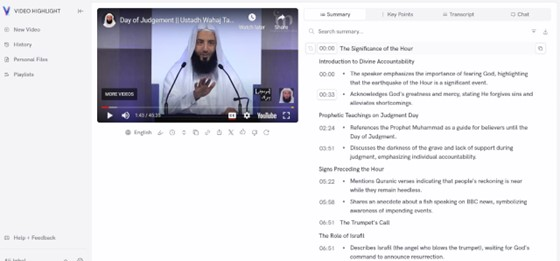
\includegraphics[width=1.1\textwidth]{figure_a.jpg}  
    \caption[Video Highlight Limitations]{Video Highlight fails to give clickable timestamps and doesn’t generate highlights in the form of a video.}
    \label{fig:video_highlight_limitations} 
\end{figure}

\begin{figure}[h]
    \centering
    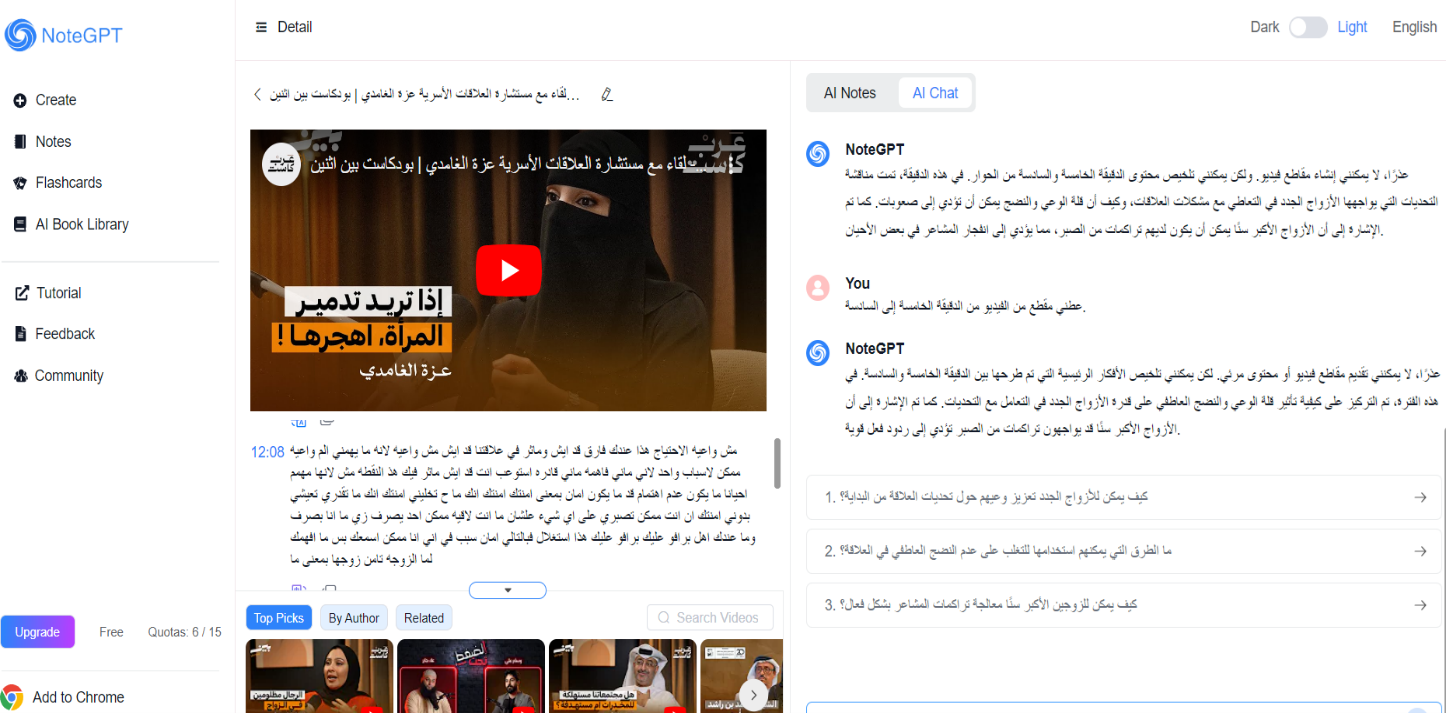
\includegraphics[width=1.1\textwidth]{figure_e.png}  
    \caption[NoteGPT Limitations]{NoteGPT doesn't generate video highlights.}
    \label{fig:notegpt_limitations}
\end{figure}

\begin{figure}[h]
    \centering
    
\includegraphics[width=1.1\textwidth]{figure_d.png}  
    \caption[Gistly Limitations]{Gistly does not have the option to chat with the application.}
    \label{fig:gistly_limitations}
\end{figure}

\begin{figure}[h]
    \centering
    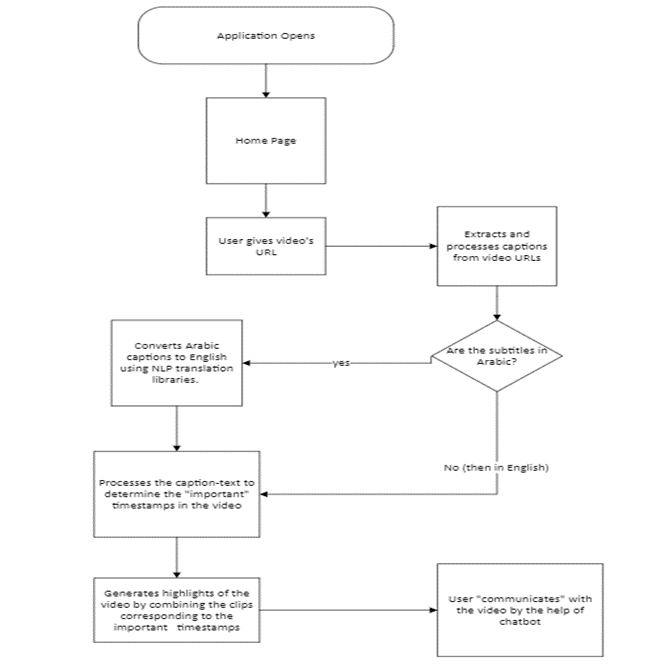
\includegraphics[width=1.0\textwidth]{figure_f.png}  
    \caption[Proposed System Architecture]{Proposed System Architecture\\
    The architecture outlines the workflow of VidSense, beginning with user input (video URL) and progressing through caption extraction, NLP processing, sentiment analysis, and video segmentation. Each component interacts to deliver precise, sentiment-enriched video highlights while supporting multilingual capabilities.}
    \label{fig:proposed_system_architecture}
\end{figure}




\end{document}
